\documentclass[aspectratio=169]{beamer}
\usetheme{Warsaw}
\usecolortheme{uiowa}
\useoutertheme[subsection=true]{smoothbars}
\usepackage{amsmath,amssymb}
\usepackage{pgfplots}
\pgfplotsset{compat=1.18}
\input{custom.tex}

\title[STAT 2020 Week 12 \hfill \insertframenumber/\inserttotalframenumber]{STAT 2020 Discussion Slides}
\subtitle{Week 12: Parameters vs. Statistics and CI for Mean (sigma known)}
\author{Shuo Li}
\institute{University of Iowa}
\date{\today}
\logo{
\includegraphics[width=0.12\textwidth]{iowa-logo.png}}

\begin{document}

\begin{frame}
  \titlepage
\end{frame}

\begin{frame}{Index (Outline)}
  \tableofcontents[hideallsubsections]
\end{frame}

% ==============================
\section{Week 12 Goals}
% ==============================

\subsection{Agenda}
\begin{frame}{Agenda}
  \begin{itemize}
    \item Distinguish population parameters vs. sample statistics
    \item Compute sample mean and sample standard deviation
    \item Interpret five-number summary from a boxplot
    \item Build CI for mean when \(\sigma^2\) is known
    \item Check if a candidate value is reasonable using CI
    \item Margin of error, interval width, and required sample size
    \item Attendance check
  \end{itemize}
\end{frame}

% ==============================
\section{Parameters vs. Statistics}
% ==============================

\subsection{Core Definitions}
\begin{frame}{Parameter vs. Statistic}
  \textbf{Parameter:} a fixed (usually unknown) population value.
  \[
    \mu,\ \sigma^2,\ p
  \]

  \textbf{Statistic:} a quantity computed from sample data.
  \[
    \bar X,\ S^2,\ \hat p
  \]

  \vspace{2mm}
  Key distinction:
  \begin{itemize}
    \item Parameter describes the population.
    \item Statistic changes from sample to sample.
  \end{itemize}
\end{frame}

\subsection{Computation Refresher}
\begin{frame}{Sample Mean and Sample SD}
  Given data \(X_1,\dots,X_n\):
  \[
    \bar X=\frac{1}{n}\sum_{i=1}^n X_i,
    \qquad
    S^2=\frac{1}{n-1}\sum_{i=1}^n (X_i-\bar X)^2,
    \qquad
    S=\sqrt{S^2}.
  \]

  \vspace{2mm}
  \textbf{Reminder:}
  \begin{itemize}
    \item Use \(n-1\) in sample variance for unbiased estimation.
    \item Calculator output often reports both \(S\) and \(S_x\): use sample SD.
  \end{itemize}
\end{frame}

\subsection{Plot Interpretation}
\begin{frame}{Boxplot Interpretation (What to Know)}
  Students are not required to draw plots by hand, but should interpret them.

  \vspace{2mm}
  From a boxplot, identify:
  \begin{itemize}
    \item Minimum
    \item First quartile \(Q_1\)
    \item Median
    \item Third quartile \(Q_3\)
    \item Maximum
  \end{itemize}

  \vspace{2mm}
  Also comment on:
  \begin{itemize}
    \item Possible skewness
    \item Potential outliers
  \end{itemize}
\end{frame}

\subsection{Worked Boxplot Example}
\begin{frame}{Boxplot Example: Read and Interpret}
  \centering
  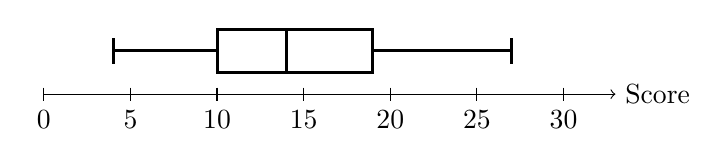
\begin{tikzpicture}[x=0.22cm,y=0.55cm]
    \draw[->] (0,0) -- (33,0) node[right] {Score};
    \foreach \x in {0,5,10,15,20,25,30}
      \draw (\x,0.15) -- (\x,-0.15) node[below] {\x};

    % Example five-number summary: min=4, Q1=10, median=14, Q3=19, max=27
    \draw[line width=1.1pt] (4,1) -- (10,1);
    \draw[line width=1.1pt] (19,1) -- (27,1);
    \draw[line width=1.1pt] (10,0.5) rectangle (19,1.5);
    \draw[line width=1.1pt] (14,0.5) -- (14,1.5);
    \draw[line width=1.1pt] (4,0.7) -- (4,1.3);
    \draw[line width=1.1pt] (27,0.7) -- (27,1.3);
  \end{tikzpicture}

  \vspace{1mm}
  Five-number summary: \((4,10,14,19,27)\)

  \vspace{1mm}
  \begin{itemize}
    \item Middle 50\% lies between \(Q_1=10\) and \(Q_3=19\).
    \item \(\mathrm{IQR}=Q_3-Q_1=9\).
    \item Right whisker is slightly longer, suggesting mild right skew.
  \end{itemize}
\end{frame}

\subsection{Quick Identification Drill}
\begin{frame}{Quick Drill: Parameter or Statistic?}
  Classify each quantity:
  \begin{enumerate}
    \item \(\mu\): true average GPA of all STAT 2020 students this semester
    \item \(\bar X\): average GPA of 40 sampled students
    \item \(p\): true proportion of students who attended every discussion
    \item \(\hat p\): proportion from this week's sampled section
  \end{enumerate}
  \pause
  \textbf{Answer:}
  \begin{itemize}
    \item (1), (3) are parameters.
    \item (2), (4) are statistics.
  \end{itemize}
\end{frame}

% ==============================
\section{CI for Mean (sigma known)}
% ==============================

\subsection{When to Use This CI}
\begin{frame}{Conditions for CI of \(\mu\) with Known \(\sigma\)}
  CI formula for \(\mu\) with known population SD \(\sigma\):
  \[
    \bar X \pm z_{\alpha/2}\frac{\sigma}{\sqrt{n}}.
  \]

  \vspace{2mm}
  Conditions in this course:
  \begin{itemize}
    \item If population is normal: formula is valid for any \(n\).
    \item If population is non-normal: use when \(n\ge 30\).
  \end{itemize}
\end{frame}

\subsection{Notation Reminder}
\begin{frame}{Notation Reminder: \(z_p\)}
  To avoid confusion with earlier topics:
  \begin{itemize}
    \item Earlier convention: \(z_p\) was the lower-tail quantile, \(P(Z\le z_p)=p\).
    \item This week: \(z_p\) is the upper-tail critical value, \(P(Z>z_p)=p\).
  \end{itemize}

  \vspace{1mm}
  So in this chapter:
  \[
    z_{0.025}=1.96
    \quad\text{(same number as lower-tail }z_{0.975}\text{).}
  \]
\end{frame}

\subsection{Main Formula}
\begin{frame}{CI Formula and Structure}
  A \((1-\alpha)100\%\) CI is
  \[
    (a,b)=\left(\bar X-z_{\alpha/2}\frac{\sigma}{\sqrt{n}},\ \bar X+z_{\alpha/2}\frac{\sigma}{\sqrt{n}}\right).
  \]

  \vspace{2mm}
  In class/exams, it is enough to report:
  \[
    \text{95\% CI for }\mu\text{ is }(a,b).
  \]

  \vspace{1mm}
  (No long interpretation paragraph is required.)
\end{frame}

\subsection{Worked Example}
\begin{frame}{Example: Compute a 95\% CI}
  Suppose \(\bar X=82\), \(\sigma=12\), \(n=36\), normal population.

  \[
    \SE(\bar X)=\frac{12}{\sqrt{36}}=2,
    \qquad
    z_{0.025}=1.96.
  \]
  \[
    \ME=1.96\times 2=3.92.
  \]
  \[
    \text{95\% CI: }82\pm 3.92=(78.08,\ 85.92).
  \]
\end{frame}

\subsection{Reasonable Value Check}
\begin{frame}{Is a Value Reasonable for \(\mu\)?}
  Rule used in discussion:
  \begin{itemize}
    \item If candidate \(\mu_0\in(a,b)\): reasonable.
    \item If candidate \(\mu_0\notin(a,b)\): not reasonable at that confidence level.
  \end{itemize}

  \vspace{2mm}
  Example from previous CI \((78.08,85.92)\):
  \begin{itemize}
    \item \(\mu_0=80\): reasonable.
    \item \(\mu_0=90\): not reasonable.
  \end{itemize}
\end{frame}

% ==============================
\section{Margin of Error and Sample Size}
% ==============================

\subsection{Key Quantities}
\begin{frame}{Margin of Error and Width}
  For known \(\sigma\):
  \[
    \ME = z_{\alpha/2}\frac{\sigma}{\sqrt{n}},
    \qquad
    \text{Width}=2\times \ME.
  \]

  \vspace{2mm}
  Consequences:
  \begin{itemize}
    \item Larger \(n\) \(\Rightarrow\) smaller \(\ME\), narrower CI.
    \item Larger confidence level \(\Rightarrow\) larger \(z_{\alpha/2}\), wider CI.
    \item Larger \(\sigma\) \(\Rightarrow\) wider CI.
  \end{itemize}
\end{frame}

\subsection{Solve for Required n}
\begin{frame}{Required Sample Size from Target Width}
  Want CI width at most \(W\):
  \[
    2z_{\alpha/2}\frac{\sigma}{\sqrt{n}}\le W.
  \]
  Solve:
  \[
    n\ge \left(\frac{2z_{\alpha/2}\sigma}{W}\right)^2.
  \]

  \vspace{2mm}
  Always round \textbf{up} to the next integer.
\end{frame}

\subsection{Sample Size Example}
\begin{frame}{Example: Width Requirement}
  Suppose \(\sigma=12\), confidence 95\% \((z_{0.025}=1.96)\),
  and require width \(W\le 4\).

  \[
    n\ge \left(\frac{2(1.96)(12)}{4}\right)^2
    =11.76^2
    =138.30.
  \]
  Minimum integer sample size:
  \[
    n=139.
  \]
\end{frame}

\subsection{Special Note}
\begin{frame}{When CI May Be Unnecessary}
  In some parametric settings, the true mean \(\mu\) may already be known
  once the model parameter is given.

  \vspace{2mm}
  Then constructing a CI for \(\mu\) may be unnecessary for that question.

  \vspace{2mm}
  Use CI when \(\mu\) is unknown and needs estimation from sample data.
\end{frame}

% ==============================
\section{Practice (Quick Drills)}
% ==============================

\subsection{Practice 1}
\begin{frame}{Practice 1: Compute CI Quickly}
  Given \(\bar X=84\), \(\sigma=10\), \(n=25\), find a 95\% CI for \(\mu\).
  \pause
  \[
    \SE=\frac{10}{5}=2,
    \quad
    \ME=1.96(2)=3.92,
  \]
  \[
    \text{CI}=84\pm 3.92=(80.08,\ 87.92).
  \]
\end{frame}

\subsection{Practice 2}
\begin{frame}{Practice 2: Required \(n\)}
  If \(\sigma=15\), confidence is 90\% \((z_{0.05}=1.645)\),
  and target width is at most \(6\), find minimum \(n\).
  \pause
  \[
    n\ge\left(\frac{2(1.645)(15)}{6}\right)^2
    =8.225^2
    =67.65.
  \]
  \[
    n=68.
  \]
\end{frame}

\subsection{Practice 3}
\begin{frame}{Practice 3: Reasonable or Not?}
  A 95\% CI for \(\mu\) is \((21.2,24.8)\).

  Is \(\mu_0=25\) reasonable?
  \pause

  \[
    25\notin(21.2,24.8)
    \quad\Rightarrow\quad
    \text{not reasonable at 95\% level.}
  \]
\end{frame}

% ==============================
\section{Wrap-Up}
% ==============================

\subsection{Take-Home Messages}
\begin{frame}{Take-Home Messages}
  \begin{itemize}
    \item Separate parameters (population) from statistics (sample).
    \item For CI of \(\mu\) with known \(\sigma\), check conditions first.
    \item CI width equals \(2\times\ME\).
    \item Use CI membership to judge whether a candidate \(\mu\) is reasonable.
    \item For target width, solve for \(n\) and round up.
  \end{itemize}
\end{frame}

% ==============================
\section{Attendance Check}
% ==============================

\begin{frame}{In-Class Attendance Check (Quick)}
  Suppose \(\bar X=52\), \(\sigma=16\), \(n=64\).

  \vspace{1mm}
  1) Construct the 95\% CI for \(\mu\).\\
  2) Is \(\mu_0=55\) a reasonable value?

  \vspace{3mm}
  \textit{Please submit: Full Name; Section Number; Your Answer}

  \pause
  \vspace{2mm}
  \textbf{Answer:}
  \[
    \SE=\frac{16}{\sqrt{64}}=2,
    \quad
    \ME=1.96(2)=3.92,
  \]
  \[
    \text{CI}=52\pm3.92=(48.08,55.92),
    \quad
    55\in(48.08,55.92).
  \]
  So \(\mu_0=55\) is reasonable.
\end{frame}

\end{document}



